\documentclass{standalone}
\usepackage{tikz}
\usetikzlibrary{patterns, positioning}

\begin{document}
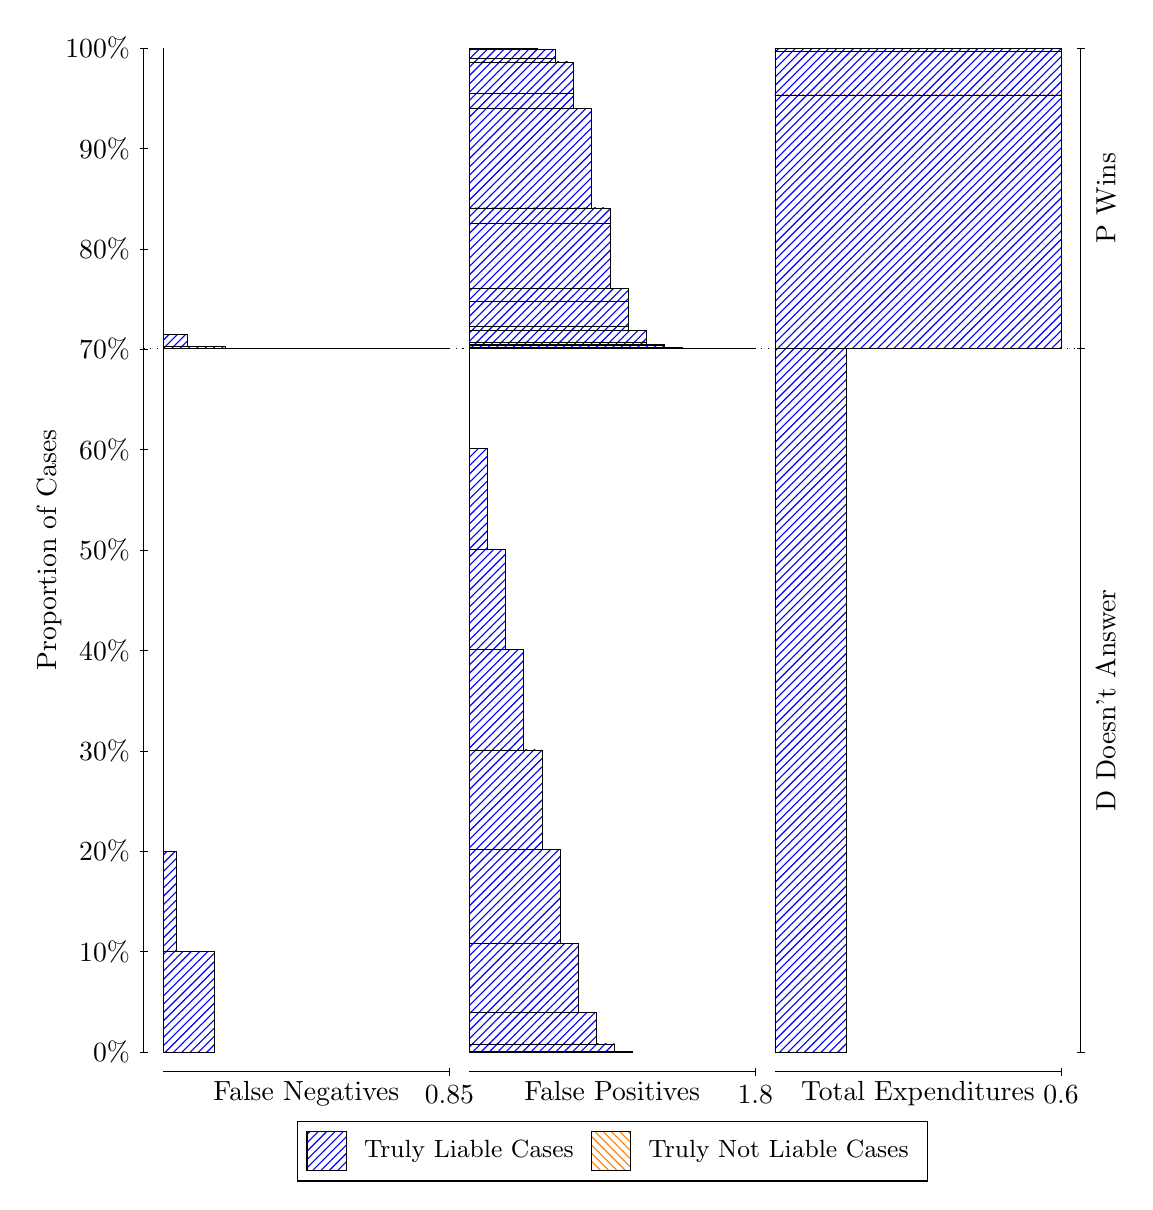
\begin{tikzpicture}
\draw[black, very thin] (1.5,1.75) -- (1.5,14.5);
\node[rotate=90, anchor=center] at (0.3, 8.125) {Proportion of Cases};
\draw[black, very thin] (1.45,1.75) -- (1.55,1.75);
\node[anchor=east] at (1.45, 1.75) {0\%};
\draw[black, very thin] (1.45,3.025) -- (1.55,3.025);
\node[anchor=east] at (1.45, 3.025) {10\%};
\draw[black, very thin] (1.45,4.3) -- (1.55,4.3);
\node[anchor=east] at (1.45, 4.3) {20\%};
\draw[black, very thin] (1.45,5.575) -- (1.55,5.575);
\node[anchor=east] at (1.45, 5.575) {30\%};
\draw[black, very thin] (1.45,6.85) -- (1.55,6.85);
\node[anchor=east] at (1.45, 6.85) {40\%};
\draw[black, very thin] (1.45,8.125) -- (1.55,8.125);
\node[anchor=east] at (1.45, 8.125) {50\%};
\draw[black, very thin] (1.45,9.4) -- (1.55,9.4);
\node[anchor=east] at (1.45, 9.4) {60\%};
\draw[black, very thin] (1.45,10.675) -- (1.55,10.675);
\node[anchor=east] at (1.45, 10.675) {70\%};
\draw[black, very thin] (1.45,11.95) -- (1.55,11.95);
\node[anchor=east] at (1.45, 11.95) {80\%};
\draw[black, very thin] (1.45,13.225) -- (1.55,13.225);
\node[anchor=east] at (1.45, 13.225) {90\%};
\draw[black, very thin] (1.45,14.5) -- (1.55,14.5);
\node[anchor=east] at (1.45, 14.5) {100\%};

\draw[black, very thin] (13.4,1.75) -- (13.4,14.5);
\draw[black, very thin] (13.35,1.75) -- (13.45,1.75);
\node[anchor=west] at (13.35, 1.75) {};
\draw[black, very thin] (13.35,10.687) -- (13.45,10.687);
\node[anchor=west] at (13.35, 10.687) {};
\draw[black, very thin] (13.35,14.5) -- (13.45,14.5);
\node[anchor=west] at (13.35, 14.5) {};

\draw[black, very thin, pattern color=blue, pattern=north east lines] (1.75,1.75) rectangle (2.3912,3.025);
\draw[black, very thin, pattern color=blue, pattern=north east lines] (1.75,3.025) rectangle (1.9162,4.3);
\draw[black, very thin, pattern color=orange, pattern=north west lines] (1.75,4.3) rectangle (1.75,4.3);
\draw[black, very thin, pattern color=blue, pattern=north east lines] (1.75,4.3) rectangle (1.75,10.687);
\draw[black, very thin, pattern color=blue, pattern=north east lines] (1.75,10.687) rectangle (5.3833,10.687);
\draw[black, very thin, pattern color=blue, pattern=north east lines] (1.75,10.687) rectangle (4.9084,10.687);
\draw[black, very thin, pattern color=blue, pattern=north east lines] (1.75,10.687) rectangle (4.4334,10.687);
\draw[black, very thin, pattern color=blue, pattern=north east lines] (1.75,10.687) rectangle (3.9585,10.687);
\draw[black, very thin, pattern color=blue, pattern=north east lines] (1.75,10.687) rectangle (3.9585,10.687);
\draw[black, very thin, pattern color=blue, pattern=north east lines] (1.75,10.687) rectangle (3.4836,10.687);
\draw[black, very thin, pattern color=blue, pattern=north east lines] (1.75,10.687) rectangle (3.4836,10.687);
\draw[black, very thin, pattern color=blue, pattern=north east lines] (1.75,10.687) rectangle (3.4836,10.687);
\draw[black, very thin, pattern color=blue, pattern=north east lines] (1.75,10.687) rectangle (3.0086,10.687);
\draw[black, very thin, pattern color=blue, pattern=north east lines] (1.75,10.687) rectangle (3.0086,10.688);
\draw[black, very thin, pattern color=blue, pattern=north east lines] (1.75,10.688) rectangle (2.5337,10.688);
\draw[black, very thin, pattern color=blue, pattern=north east lines] (1.75,10.688) rectangle (2.5337,10.688);
\draw[black, very thin, pattern color=blue, pattern=north east lines] (1.75,10.688) rectangle (2.5337,10.706);
\draw[black, very thin, pattern color=blue, pattern=north east lines] (1.75,10.706) rectangle (2.0587,10.707);
\draw[black, very thin, pattern color=blue, pattern=north east lines] (1.75,10.707) rectangle (2.0587,10.863);
\draw[black, very thin, pattern color=blue, pattern=north east lines] (1.75,10.863) rectangle (2.0587,10.863);
\draw[black, very thin, pattern color=orange, pattern=north west lines] (1.75,10.863) rectangle (1.75,10.863);
\draw[black, very thin, pattern color=blue, pattern=north east lines] (1.75,10.863) rectangle (1.75,14.5);
\draw[black, very thin, pattern color=orange, pattern=north west lines] (5.6333,1.75) rectangle (7.7095,1.75);
\draw[black, very thin, pattern color=blue, pattern=north east lines] (5.6333,1.75) rectangle (7.7095,1.7614);
\draw[black, very thin, pattern color=blue, pattern=north east lines] (5.6333,1.7614) rectangle (7.4788,1.8527);
\draw[black, very thin, pattern color=blue, pattern=north east lines] (5.6333,1.8527) rectangle (7.2481,2.2486);
\draw[black, very thin, pattern color=blue, pattern=north east lines] (5.6333,2.2486) rectangle (7.0175,3.1304);
\draw[black, very thin, pattern color=blue, pattern=north east lines] (5.6333,3.1304) rectangle (6.7868,4.3202);
\draw[black, very thin, pattern color=blue, pattern=north east lines] (5.6333,4.3202) rectangle (6.5561,5.5873);
\draw[black, very thin, pattern color=blue, pattern=north east lines] (5.6333,5.5873) rectangle (6.3254,6.862);
\draw[black, very thin, pattern color=blue, pattern=north east lines] (5.6333,6.862) rectangle (6.0947,8.137);
\draw[black, very thin, pattern color=blue, pattern=north east lines] (5.6333,8.137) rectangle (5.864,9.412);
\draw[black, very thin, pattern color=blue, pattern=north east lines] (5.6333,9.412) rectangle (5.6333,10.687);
\draw[black, very thin, pattern color=orange, pattern=north west lines] (5.6333,10.687) rectangle (9.2667,10.687);
\draw[black, very thin, pattern color=blue, pattern=north east lines] (5.6333,10.687) rectangle (9.2667,10.687);
\draw[black, very thin, pattern color=orange, pattern=north west lines] (5.6333,10.687) rectangle (9.036,10.687);
\draw[black, very thin, pattern color=blue, pattern=north east lines] (5.6333,10.687) rectangle (9.036,10.687);
\draw[black, very thin, pattern color=orange, pattern=north west lines] (5.6333,10.687) rectangle (8.8053,10.687);
\draw[black, very thin, pattern color=blue, pattern=north east lines] (5.6333,10.687) rectangle (8.8053,10.687);
\draw[black, very thin, pattern color=blue, pattern=north east lines] (5.6333,10.687) rectangle (8.5746,10.687);
\draw[black, very thin, pattern color=orange, pattern=north west lines] (5.6333,10.687) rectangle (8.5746,10.687);
\draw[black, very thin, pattern color=blue, pattern=north east lines] (5.6333,10.687) rectangle (8.5746,10.688);
\draw[black, very thin, pattern color=orange, pattern=north west lines] (5.6333,10.688) rectangle (8.3439,10.688);
\draw[black, very thin, pattern color=blue, pattern=north east lines] (5.6333,10.688) rectangle (8.3439,10.691);
\draw[black, very thin, pattern color=blue, pattern=north east lines] (5.6333,10.691) rectangle (8.3439,10.694);
\draw[black, very thin, pattern color=orange, pattern=north west lines] (5.6333,10.694) rectangle (8.1132,10.694);
\draw[black, very thin, pattern color=blue, pattern=north east lines] (5.6333,10.694) rectangle (8.1132,10.727);
\draw[black, very thin, pattern color=blue, pattern=north east lines] (5.6333,10.727) rectangle (8.1132,10.734);
\draw[black, very thin, pattern color=blue, pattern=north east lines] (5.6333,10.734) rectangle (7.8825,10.769);
\draw[black, very thin, pattern color=orange, pattern=north west lines] (5.6333,10.769) rectangle (7.8825,10.769);
\draw[black, very thin, pattern color=blue, pattern=north east lines] (5.6333,10.769) rectangle (7.8825,10.918);
\draw[black, very thin, pattern color=blue, pattern=north east lines] (5.6333,10.918) rectangle (7.6519,10.962);
\draw[black, very thin, pattern color=orange, pattern=north west lines] (5.6333,10.962) rectangle (7.6519,10.962);
\draw[black, very thin, pattern color=blue, pattern=north east lines] (5.6333,10.962) rectangle (7.6519,11.286);
\draw[black, very thin, pattern color=blue, pattern=north east lines] (5.6333,11.286) rectangle (7.6519,11.452);
\draw[black, very thin, pattern color=orange, pattern=north west lines] (5.6333,11.452) rectangle (7.4212,11.452);
\draw[black, very thin, pattern color=blue, pattern=north east lines] (5.6333,11.452) rectangle (7.4212,12.273);
\draw[black, very thin, pattern color=blue, pattern=north east lines] (5.6333,12.273) rectangle (7.4212,12.468);
\draw[black, very thin, pattern color=blue, pattern=north east lines] (5.6333,12.468) rectangle (7.4212,12.469);
\draw[black, very thin, pattern color=orange, pattern=north west lines] (5.6333,12.469) rectangle (7.1905,12.469);
\draw[black, very thin, pattern color=blue, pattern=north east lines] (5.6333,12.469) rectangle (7.1905,13.729);
\draw[black, very thin, pattern color=blue, pattern=north east lines] (5.6333,13.729) rectangle (7.1905,13.729);
\draw[black, very thin, pattern color=blue, pattern=north east lines] (5.6333,13.729) rectangle (6.9598,13.924);
\draw[black, very thin, pattern color=blue, pattern=north east lines] (5.6333,13.924) rectangle (6.9598,14.324);
\draw[black, very thin, pattern color=blue, pattern=north east lines] (5.6333,14.324) rectangle (6.9598,14.324);
\draw[black, very thin, pattern color=blue, pattern=north east lines] (5.6333,14.324) rectangle (6.7291,14.368);
\draw[black, very thin, pattern color=blue, pattern=north east lines] (5.6333,14.368) rectangle (6.7291,14.48);
\draw[black, very thin, pattern color=blue, pattern=north east lines] (5.6333,14.48) rectangle (6.7291,14.481);
\draw[black, very thin, pattern color=blue, pattern=north east lines] (5.6333,14.481) rectangle (6.4984,14.484);
\draw[black, very thin, pattern color=blue, pattern=north east lines] (5.6333,14.484) rectangle (6.4984,14.499);
\draw[black, very thin, pattern color=blue, pattern=north east lines] (5.6333,14.499) rectangle (6.4984,14.499);
\draw[black, very thin, pattern color=blue, pattern=north east lines] (5.6333,14.499) rectangle (6.4984,14.499);
\draw[black, very thin, pattern color=blue, pattern=north east lines] (5.6333,14.499) rectangle (6.2677,14.5);
\draw[black, very thin, pattern color=blue, pattern=north east lines] (5.6333,14.5) rectangle (6.2677,14.5);
\draw[black, very thin, pattern color=blue, pattern=north east lines] (5.6333,14.5) rectangle (6.037,14.5);
\draw[black, very thin, pattern color=blue, pattern=north east lines] (5.6333,14.5) rectangle (6.037,14.5);
\draw[black, very thin, pattern color=blue, pattern=north east lines] (5.6333,14.5) rectangle (5.8063,14.5);
\draw[black, very thin, pattern color=blue, pattern=north east lines] (5.6333,14.5) rectangle (5.8063,14.5);
\draw[black, very thin, pattern color=blue, pattern=north east lines] (5.6333,14.5) rectangle (5.6333,14.5);
\draw[black, very thin, pattern color=orange, pattern=north west lines] (9.5167,1.75) rectangle (10.425,1.75);
\draw[black, very thin, pattern color=blue, pattern=north east lines] (9.5167,1.75) rectangle (10.425,10.687);
\draw[black, very thin, pattern color=orange, pattern=north west lines] (9.5167,10.687) rectangle (13.15,10.687);
\draw[black, very thin, pattern color=blue, pattern=north east lines] (9.5167,10.687) rectangle (13.15,13.906);
\draw[black, very thin, pattern color=orange, pattern=north west lines] (9.5167,13.906) rectangle (13.15,13.906);
\draw[black, very thin, pattern color=blue, pattern=north east lines] (9.5167,13.906) rectangle (13.15,14.455);
\draw[black, very thin, pattern color=orange, pattern=north west lines] (9.5167,14.455) rectangle (13.15,14.455);
\draw[black, very thin, pattern color=blue, pattern=north east lines] (9.5167,14.455) rectangle (13.15,14.5);
\draw[black, dotted] (1.5,10.687) -- (13.4,10.687);
\draw[black, very thin] (1.75,1.5) -- (5.3833,1.5);
\node[anchor=north] at (3.5667, 1.5) {False Negatives};
\draw[black, very thin] (5.3833,1.45) -- (5.3833,1.55);
\node[anchor=north] at (5.3833, 1.45) {0.85};

\draw[black, very thin] (5.6333,1.5) -- (9.2667,1.5);
\node[anchor=north] at (7.45, 1.5) {False Positives};
\draw[black, very thin] (9.2667,1.45) -- (9.2667,1.55);
\node[anchor=north] at (9.2667, 1.45) {1.8};

\draw[black, very thin] (9.5167,1.5) -- (13.15,1.5);
\node[anchor=north] at (11.333, 1.5) {Total Expenditures};
\draw[black, very thin] (13.15,1.45) -- (13.15,1.55);
\node[anchor=north] at (13.15, 1.45) {0.6};

\node[black, centered, rotate=90] at (13.72, 6.2185) {D Doesn't Answer};
\node[black, centered, rotate=90] at (13.72, 12.594) {P Wins};

\draw (7.449999999999999,1.5) node[draw=none] (baseCoordinate) {};
\begin{scope}[align=center]
        \matrix[scale=0.5, draw=black, below=0.5cm of baseCoordinate, nodes={draw}, column sep=0.1cm]{
            \node[rectangle, draw, minimum width=0.5cm, minimum height=0.5cm, pattern=north east lines, pattern color=blue] {}; &
            \node[draw=none, font=\small] (B) {Truly Liable Cases}; &
            \node[rectangle, draw, minimum width=0.5cm, minimum height=0.5cm, pattern=north west lines, pattern color=orange] {}; &
            \node[draw=none, font=\small] (B) {Truly Not Liable Cases}; \\
            };
\end{scope}

\end{tikzpicture}
\end{document}